\chapter{Summary and Outlook}\label{cha:SummaryOutlook}
This chapter begins by giving a summary of the topics discussed in this thesis in section \ref{sec:summary}. Then, section \ref{sec:outlook} gives an outlook for future research works in synthetic dataset generation for plant disease monitoring tasks.


% ✅✅✅✅
\section{Summary}\label{sec:summary}
This bachelor thesis aimed to determine whether image processing techniques can be used as augmentation techniques to generate more datasets for training disease detection models for precision farming. Previous research showed that basic augmentation techniques like random cropping and rotation were used to increase the training dataset to prevent the problem of overfitting. However, this study is the first known to use the proposed approach to create a synthetic plant disease dataset using image processing techniques from two different plant images. Furthermore, the result of this study confirmed that new datasets could be generated using the proposed techniques.

The results of the trained models using the synthetically generated images in this research showed the tremendous result of the proposed techniques. The proposed approach is an excellent step by step guide that can be used to synthetically generate an arbitrary number of image datasets using healthy and diseased leaf images. Likewise, this approach of dataset generation can significantly reduce the time needed to acquire a dataset for plant disease model training.

% It can be seen in figure \ref{fig:my_gen_7} that some of the leaves have little or no disease falling on them. This occurrence is mainly attributed to the fact that the portion and orientation of the disease areas were not uniform throughout the images in the diseased leaves dataset. Nevertheless, the following steps will be to improve the proposed approach to ensure that the disease is intelligently placed on the leaf areas irrespective of the diversities in the desired disease and plant leaf dataset.

% One of the reasons for performing this experiment was to see if a synthetic disease dataset can be created for any arbitrary plant using diseased images of plants known to occur in other plants. Based on the experiment results, it is safe to say that this approach of creating a synthetic dataset is possible.

This thesis has described a complete approach for generating synthetic disease image datasets for sugar beet plants. The proposed approach builds upon ideas in image processing to provide a general, easy to use method for generating synthetic images. The main contribution is the extraction of the disease sections in diseased plant images and concatenating them on the leaf surface of healthy leaves. The thesis began by highlighting the problem statement of the research work and precision farming regarding disease monitoring and detection. Then we explained the relevant theories in image processing used to augment insufficient datasets in sugar beet. Likewise, we reviewed research papers in precision farming geared towards plant disease detection and monitoring. Finally, the results from the experiments were presented and analysed with the generated fake images.

\section{Outlook}\label{sec:outlook}
% This section presents the limitations of the proposed approach, and the next section discusses future work and open issues. 
% The proposed approach has several limitations, which are discussed below. 

Although the proposed approach produced tremendous results, there were some shortcomings worth noting.

It can be seen in figure \ref{fig:my_gen_7} that some of the leaves have little or no disease falling on them. This occurrence is mainly attributed to the different orientations in the sugar beet leaf area and disease areas in the images making it difficult to orient them vertically. Likewise, some of the images in the sugar beet dataset had more than two leaves which increased the complexity in re-orienting.

Furthermore, the segmented disease image dataset used for synthetic image generation has some challenging images, as shown in figure \ref{fig:my_bad_seg_img}. It can be seen that some of the images in the figure have little or no disease and shadows. Likewise, images 85 and 315 in figure \ref{fig:my_bad_seg_img} are not helpful due to the greyish colour in more than half of the image area. These sorts of images in the disease image path reduced the quality of the generated images. Therefore, it is essential to inspect the quality of base images before using them for dataset generation to avoid the limitations encountered in this experiment.


\begin{figure}[!htb]
    \centering
    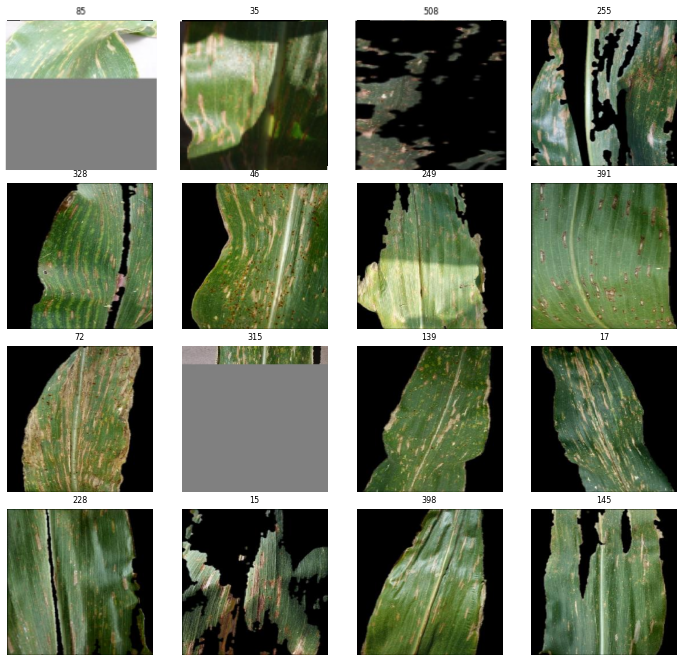
\includegraphics[scale=0.5, keepaspectratio]{Figures/notebook/bad-seg-dis.png}
    \caption{Synthetic plant leaf images generated from the PlantVillage dataset using styleGAN. \cite{arsenovic2019solving}.}
    \label{fig:my_bad_seg_img}
\end{figure} 




Based on the limitations we discussed, we can think about the following next steps to improve the proposed approach. 
An improvement on the proposed approach is to ensure that the disease is intelligently placed on the leaf areas irrespective of the diversities in the orientation angle of the desired disease and plant leaf dataset. 
% Likewise, the synthetically generated dataset from the proposed approach can be used as base images for generating more high-quality synthetic images with neural networks.

Likewise, as an extension of this research, it will be interesting to use neural network-based techniques to generate more synthetic datasets in addition to the one generated in this experiment. This technique will briefly be described using scientific references as it was not implemented in this thesis. However, the understandings from this section can be used as a foundation for implementation in future research.

% Different GAN-based architectures have been developed due to the instability in training models using standard GANs, which often result in ridiculous output by the generator network \cite{radford2015unsupervised}. Therefore, researchers have proposed using other GANs based architectures to create synthetic image datasets to augment currently limited available datasets for training purposes. For example,  Gandhi et al. \cite{gandhi2018plant} used deep convolutional GAN (DCGAN \cite{radford2015unsupervised}) for creating synthetic images to augment the limited number of local images available for training disease detection models for plants in India. Likewise, Barth et al. \cite{barth2020optimising} in their experiment used Cycle GAN for creating 10 500 synthetic images of bell pepper for their segmentation task, Zhu et al. \cite{zhu2018data} created synthetic images from the CVPPP 2017 LSC plant dataset using conditional GAN (CGAN).

Of all the GAN-based architecture documented in research papers for creating synthetic plant disease images, styleGAN has proven to have the best result \cite{arsenovic2019solving}. StyleGAN proposed by Karras et al. \cite{karras2019style} combines their previously proposed progressively growing GAN (ProGAN \cite{karras2017progressive}) and neural style transfer (NST \cite{gatys2015neural}) for creating higher resolution (up to 1024 x 1024 pixels) images with features close to the plant leaves. One of the significant advantages of styleGAN over standard GAN is its ability to influence details in the style of generated images by changing the values of the style vectors and noise of the network.


The StyleGAN architecture uses its discriminator and generator network to progressively generate synthetic images from a very resolution (4 x 4 pixels) until it reaches the desired target image resolution. The incremental learning allows the network to learn more details about the original images over time. StyleGAN replaces the nearest neighbour upsampling layers in the original ProGAN architecture with bilinear sampling. It also uses eight fully connected layers with 512 neurons to process its initial random input.

Figure \ref{fig:my_style_gan} shows the 256 x 256 pixels synthetic images generated from the PlantVillage dataset by Arsenovic et al. \cite{arsenovic2019solving} using styleGAN. Based on the resulting images, it can be concluded that styleGAN can be used for generating more synthetic images from the ones created in this thesis.

\begin{figure}[!htb]
    \centering
    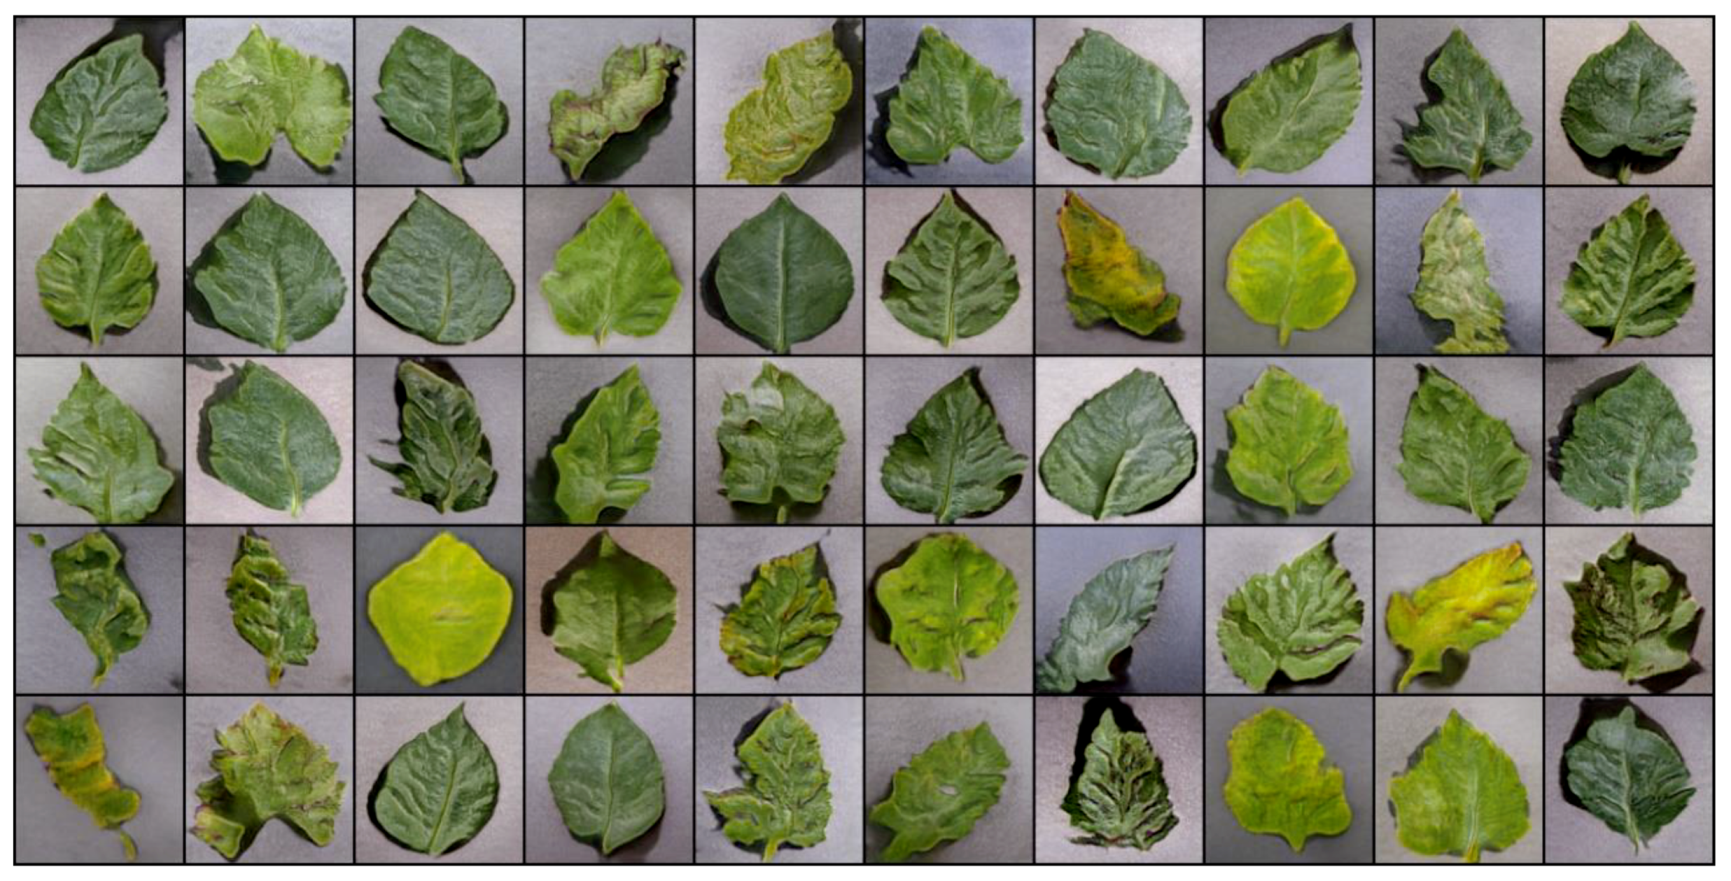
\includegraphics[scale=2, keepaspectratio]{Figures/styleGAN.png}
    \caption{Synthetic plant leaf images generated from the PlantVillage dataset using styleGAN. \cite{arsenovic2019solving}.}
    \label{fig:my_style_gan}
\end{figure} 

